\documentclass[11pt,oneside,UTF8,a4paper]{ctexbook}

%\usepackage{showframe} % 显示页面框架
%\usepackage{layouts}   % 显示布局参数

% 存放所有\usepackage命令
\usepackage{ctex}
\usepackage{xeCJK}
\usepackage{cite}
\usepackage{fancyhdr}	% 导入 fancyhdr 宏包以自定义页眉和页脚

\usepackage[T1]{fontenc} % 保证英文字体加粗有效

\usepackage{titlesec}                       % 控制标题的宏包
\usepackage{titletoc}                       % 控制目录的宏包
\usepackage{caption}
\usepackage{subcaption} % 子图支持
\usepackage{setspace}	% 导入 setspace 宏包以设置行距
\usepackage{indentfirst}
\usepackage{geometry}
\usepackage{ragged2e}  % 实现两端对齐
\usepackage{lineno}

% \usepackage[shorthands=off, ngerman]{babel}

\usepackage{fontspec}	% 导入 fontspec 宏包以支持字体设置
\usepackage[autostyle]{csquotes}
\usepackage{pdfpages} %导入其他pdf文件并带页码，参考https://texdoc.org/serve/pdfpages.pdf/0
\usepackage{graphicx}
\usepackage{geometry}
\usepackage{ulem}
\usepackage{layout}
\usepackage{tabularray}
\usepackage{xeCJKfntef}
\usepackage{calc}
\usepackage{amsmath}
\usepackage{float}
\usepackage{booktabs}  % 三线表支持
% \usepackage{tocloft}

%引入hyperref宏包 %为了美观，取消目录内容的框选 %设置目录内容的颜色 %若只需要从目录跳转到章节，加这一行就够了	% 生成有书签的pdf及其开关

\usepackage[xetex,
	CJKbookmarks=true,
	pdfstartview=FitH,
	bookmarksnumbered=true,
	bookmarksopen=true,
	colorlinks=true,
	citecolor=black,
	linkcolor=black,
	anchorcolor=black,
	urlcolor=black
]{hyperref}

\usepackage{xparse}

% \usepackage[super,square,sort&compress,numbers]{natbib}   % 导入宏包配置（参考知识库）
% 存放页边距、行距、页眉等格式设置
%\xeCJKsetup{EmboldenFactor=1}
%\setCJKfamilyfont{zhsong}{SimSun}[AutoFakeBold]

\geometry{ 
	a4paper, 
	left=3cm, right=2.5cm, 
	top=2cm, bottom=2cm, 
}

% 设置粗宋体和粗黑体

\newCJKfontfamily{\cuheiti}[AutoFakeBold={3.17}]{SimHei}

\newcommand{\yihao}{\fontsize{26pt}{26pt}\selectfont}       % 一号, 单倍行距
\newcommand{\xiaoyi}{\fontsize{24pt}{24pt}\selectfont}      % 小一, 单倍行距
\newcommand{\erhao}{\fontsize{22pt}{1.25\baselineskip}\selectfont}       % 二号, 1.25倍行距
\newcommand{\xiaoer}{\fontsize{18pt}{18pt}\selectfont}      % 小二, 单倍行距
\newcommand{\sanhao}{\fontsize{16pt}{16pt}\selectfont}      % 三号, 单倍行距
\newcommand{\xiaosan}{\fontsize{15pt}{15pt}\selectfont}     % 小三, 单倍行距
\newcommand{\sihao}{\fontsize{14pt}{16.1pt}\selectfont}       % 四号, 单倍行距
\newcommand{\xiaosi}{\fontsize{12pt}{13.8pt}\selectfont}      % 小四, 1.15倍行距
\newcommand{\xiaoxiaosi}{\fontsize{11pt}{12.65pt}\selectfont}      % 小四, 1.15倍行距
\newcommand{\wuhao}{\fontsize{10.5pt}{10.5pt}\selectfont}   % 五号, 单倍行距
\newcommand{\xiaowu}{\fontsize{9pt}{9pt}\selectfont}        % 小五, 单倍行距

\newcommand{\upcite}[1]{\textsuperscript{\textsuperscript{\cite{#1}}}} % 上角标引用参考文献

%配置ctex样式
\ctexset {
	part/pagestyle = empty,
	chapter/pagestyle = fancy,
	chapter = {
		name={,.},
		number=\textbf{\arabic{chapter}},
		format=\xiaosi\fontspec{Arial}\bfseries\raggedright, % 追加跳转
		beforeskip = {0pt},
		afterskip={10pt},
		fixskip=true,
	},
	section = {
		name={,},
		% number=\textbf{\thechapter.\arabic{section}},
		number=\arabic{chapter}.\arabic{section},
		format=\xiaoxiaosi\fontspec{Arial}\bfseries\raggedright, % 追加跳转
		beforeskip = {0pt},
		afterskip={10pt},
		fixskip=true,
	},
	subsection = {
		name={,},
		number=\textbf{\thesection.\arabic{subsection}},
		format=\xiaoxiaosi\fontspec{Arial}\bfseries\raggedright, % 追加跳转
		beforeskip = {0pt},
		afterskip={10pt},
		fixskip=true,
	},
	subsubsection = {
		number=\textbf{\alpha{subsubsection}},
		format=\xiaoxiaosi\fontspec{Arial}\bfseries\raggedright,
		beforeskip = {0pt},
		afterskip={10pt},
		fixskip=true,
	},
  	listfigurename=List of Figure,
	listtablename=List of Table,
	figurename=Figure,
	tablename=Table,
	bibname=Reference,
	indexname=Index,
}
% 摘要页的页眉设置
\fancypagestyle{toastyle}
{
	\fancyhf{} % 清空
	\fancyhead[C]{
  		\ifodd\value{page}
     		\SansC\xiaowu Abstract
  		\else
     		\SansC\xiaowu Xi'an University of Posts and Telecommunications Final Year Project (Paper)
  		\fi
	}
	\fancyfoot[C]{\thepage}
}
% 目录页的页眉设置
\fancypagestyle{tocstyle}
{
    \fancyhf{} % 清空
    \fancyhead[C]{
  		\ifodd\value{page}
     		\SansC\xiaowu Contents
  		\else
     		\SansC\xiaowu Xi'an University of Posts and Telecommunications Final Year Project (Paper)
  		\fi
}
    \fancyfoot[C]{\thepage}
}
%图目录页的页眉设置
\fancypagestyle{lofstyle}
{
	\fancyhf{} % 清空
	\fancyhead[C]{
  		\ifodd\value{page}
	 		\SansC\xiaowu List of Figure
  		\else
	 		\SansC\xiaowu Xi'an University of Posts and Telecommunications Final Year Project (Paper)
  		\fi
	}
	\fancyfoot[C]{\thepage}
}
%表目录页的页眉设置
\fancypagestyle{lotstyle}
{
	\fancyhf{} % 清空
	\fancyhead[C]{
  		\ifodd\value{page}
	 		\SansC\xiaowu List of Table
  		\else
	 		\SansC\xiaowu Xi'an University of Posts and Telecommunications Final Year Project (Paper)
  		\fi
	}
	\fancyfoot[C]{\thepage}
}
% 正文的页眉设置
% —— 可回退的英文字体宏（优先用系统字体，找不到就退而求其次）——
\IfFontExistsTF{Arial}{%
  \newcommand{\SansA}{\fontspec{Arial}}%
}{%
  \IfFontExistsTF{TeX Gyre Heros}{\newcommand{\SansA}{\fontspec{TeX Gyre Heros}}}{\newcommand{\SansA}{\sffamily}}%
}
\IfFontExistsTF{Calibri}{%
  \newcommand{\SansC}{\fontspec{Calibri}}%
}{%
  \IfFontExistsTF{Carlito}{\newcommand{\SansC}{\fontspec{Carlito}}}{\newcommand{\SansC}{\SansA}}%
}
\renewcommand{\chaptermark}[1]{%
  \markboth{\chaptername~\thechapter.\ #1}{}%
}
% —— 页眉：偶数页固定标题，奇数页章节标题（Calibri 不在则回退）——
\fancypagestyle{fancy}{
    \fancyhead[R]{}                % 清空右页眉
	\fancyhead[L]{}                % 清空左页眉
	\fancyfoot[l]{} 			   % 清空左页脚
	\fancyfoot[r]{} 			   % 清空右页脚
    \fancyhead[C]{
  	\ifodd\value{page}
     	{\SansC\xiaowu\nouppercase{\leftmark}}
  	\else
     	\SansC\xiaowu Xi'an University of Posts and Telecommunications Final Year Project (Paper)
  	\fi
}
    \fancyfoot[C]{\footnotesize\thepage}
    \renewcommand{\headrulewidth}{0.75pt}
}
% ===== 公式编号格式设置 =====
\renewcommand{\theequation}{\thechapter-\arabic{equation}}

% ===== 图片编号格式设置 =====
\renewcommand{\thefigure}{\thechapter.\arabic{figure}}

% ===== 表格编号格式设置 =====
\renewcommand{\thetable}{\thechapter.\arabic{table}}

% ===== 图表标题格式设置 =====
\captionsetup[figure]{
    font={normalsize},           % 标题字号与正文相同（11pt）
    labelfont={},              % "Fig 2-1" 加粗
    textfont={},                 % 标题文字常规
    labelsep=space,              % 编号与标题用空格分隔
    skip=10pt,                   % 标题与图片间距10pt
    position=below,              % 标题在图片下方
    name={Figure}                   % 使用 "Figure" 而非 "图"
}
\captionsetup[table]{
    font={normalsize},
    labelfont={},
    textfont={},
    labelsep=space,
    skip=10pt,
    position=above,              % 表格标题在上方
    name={Table}
}     % 导入格式配置
% % 英文摘要环境定义（含\abstract和\keywords）
% ===== 英文摘要环境定义 =====

% 设置主字体和衬线字体
\IfFontExistsTF{Arial}{%
  \setmainfont{Arial}\setsansfont{Arial}%
}
{%
  \setmainfont{TeX Gyre Heros}\setsansfont{TeX Gyre Heros}%
}

% ===== 英文摘要环境定义 =====
\newenvironment{enabstract}{%
    \clearpage
    \thispagestyle{toastyle} % 摘要页页眉页脚样式
    \vspace*{0pt} % 顶部间距
    \begin{center}
        \bfseries\rmfamily\fontsize{14}{0}\selectfont Abstract % 设置"Abstract"为 Arial 加粗，四号字，居中
    \end{center}
    \vspace{12pt} % 标题与正文间距
    \rmfamily  % 恢复衬线字体（Arial）
    \fontsize{12}{20}\selectfont % 设置正文为 Arial 字体，小四号字
    \setlength{\baselineskip}{20pt} % 设置行距为固定值 20pt
    \setlength{\parindent}{2em} % 设置首行缩进为 2 字符
    \setlength{\parskip}{0pt} % 设置段落间距为 0
    \justifying % 设置两端对齐
}
{%
    \par
}
% ===== 关键词命令定义 =====
\newcommand{\enkeywords}[1]{%
    \par\vspace{12pt}
    \noindent
    \textbf{\fontsize{12}{20}\selectfont Keywords:} % 设置"Keywords"为加粗的 Times New Roman 字体，小四号字
    \fontsize{12}{20}\selectfont\ #1 % 关键词内容为 Times New Roman 字体，小四号字
}



         % 英文摘要环境定义
% ===== 目录设置 =====
% \setcounter{page}{3} % 目录从II开始
% ===== 设置目录标题格式 =====
\renewcommand\contentsname{%
    \vspace*{0pt}% 段前绝对间距
    \raggedright % 强制左对齐
    \fontspec{Arial}\fontsize{12pt}{12pt}\selectfont\bfseries % Arial 加粗 14pt
    Contents\par
    \vspace{10pt}% 段后间距
}

% 设置目录深度：显示到 subsection 级别（0=chapter, 1=section, 2=subsection）
\setcounter{tocdepth}{1}

% 一级标题（chapter）- 加粗 Arial，使用阿拉伯数字编号
\titlecontents{chapter}[0mm] % 左间距
{\fontspec{Arial}\fontsize{11pt}{12.65pt}\selectfont\bfseries} % 标题格式：Arial 加粗
{\thecontentslabel\quad}% 标题标志
{\bfseries} % 无序号标题
{\titlerule*[4pt]{.}\contentspage} % 指引线与页码
[\vspace{10pt}] % 段后间距10磅

% 二级标题（section）- 常规 Arial
\titlecontents{section}[0em] % 左间距（缩进）
{\fontspec{Arial}\fontsize{11pt}{12.65pt}\selectfont} % 标题格式：Arial 常规
{\thecontentslabel\quad}% 标题标志
{} % 无序号标题
{\titlerule*[4pt]{.}\contentspage} % 指引线与页码
[\vspace{10pt}] % 段后间距10磅

% 三级标题（subsection）- 常规 Arial
\titlecontents{subsection}[0em] % 左间距
{\fontspec{Arial}\fontsize{12pt}{20pt}\selectfont} % 标题格式：Arial 常规
{\thecontentslabel\quad}% 标题标志
{} % 无序号标题
{\titlerule*[4pt]{.}\contentspage} % 指引线与页码
{} % 下间距

% 四级标题（subsubsection）- 常规 Arial
\titlecontents{subsubsection}[0em] % 左间距
{\fontspec{Arial}\fontsize{12pt}{20pt}\selectfont} % 标题格式：Arial 常规
{\thecontentslabel\quad}% 标题标志
{} % 无序号标题
{\titlerule*[4pt]{.}\contentspage} % 指引线与页码
{} % 下间距
% 设置行间距为20pt
%\setlength{\parskip}{0.3\baselineskip}
\makeatletter
\def\@cite#1#2{\textsuperscript{[{#1\if@tempswa , #2\fi}]}}
\makeatother
% 自定义命令定义
\makeatletter
\def\ctitle#1{\def\@ctitle{#1}}\def\@ctitle{}
\def\etitle#1{\def\@etitle{#1}}\def\@etitle{}
\def\cdegree#1{\def\@cdegree{#1}}\def\@cdegree{}
\def\caffil#1{\def\@caffil{#1}}\def\@caffil{}
\def\csubject#1{\def\@csubject{#1}}\def\@csubject{}
\def\cgrade#1{\def\@cgrade{#1}}\def\@cgrade{}
\def\cauthor#1{\def\@cauthor{#1}}\def\@cauthor{}
\def\cnumber#1{\def\@cnumber{#1}}\def\@cnumber{}
\def\csupervisor#1{\def\@csupervisor{#1}}\def\@csupervisor{}
\def\crank#1{\def\@crank{#1}}\def\@crank{}
\def\cdate#1{\def\@cdate{#1}}\def\@cdate{}
\def\startdate#1{\def\@startdate{#1}}\def\@startdate{}
\def\enddate#1{\def\@enddate{#1}}\def\@enddate{}

% \renewcommand{\ULdepth}{4pt}		% 控制下划线与文本之间的垂直位置。
\renewcommand{\ULthickness}{1.1pt}		% 控制下划线的粗细。

\newcommand\dlmu[2][4cm]{%
	\hskip1pt\uline{\hbox to #1{\hss#2\hss}}\hskip3pt%
}

% 定义封面
\def\makecover{
    \cleardoublepage%
    \newgeometry{left=3cm, right=2.5cm, top=2cm, bottom=2cm} % 仅本页生效的新边距
    \begin{titlepage}
        % 左上角校徽（固定宽度，保持原始比例：仅给 width 即可）
        \vspace*{0pt}
        \noindent\includegraphics[width=9cm]{cover/cover1.png}

        % 中央标题与副标题
        \vspace*{20pt}
        \begin{center}
            {\bfseries\fontspec{Arial}\fontsize{36pt}{60pt}\selectfont Final Year Project (Paper)\par}

            \vspace*{48pt}
            {\bfseries\fontspec{Arial}\fontsize{18pt}{22pt}\selectfont \@etitle\par}
            {\songti\fontsize{16pt}{20pt}\selectfont \@ctitle\par}

            \vspace*{18pt}

            % 信息表
            \renewcommand\arraystretch{1.5}
            \newlength{\coverTableW}\setlength{\coverTableW}{12.5cm}
            \begin{tabular}{p{4.2cm} p{8.3cm}}
                {\bfseries\fontspec{Arial} School:} & \fontspec{Arial}\@caffil \\
                {\bfseries\fontspec{Arial} Major:} & \fontspec{Arial}\@csubject \\
                {\bfseries\fontspec{Arial} Class:} & \fontspec{Arial}\@cgrade \\
                {\bfseries\fontspec{Arial} Name:} & \fontspec{Arial}\@cauthor \\
                {\bfseries\fontspec{Arial} Student ID:} & \fontspec{Arial}\@cnumber \\
                {\bfseries\fontspec{Arial} Supervisor:} & \fontspec{Arial}\@csupervisor \\
                {\bfseries\fontspec{Arial} Professional Title:} & \fontspec{Arial}\@crank \\
                {\bfseries\fontspec{Arial} From:} &
                  \fontspec{Arial}\@startdate\quad {\bfseries To:}\quad \fontspec{Arial}\@enddate \\
            \end{tabular}
        \end{center}
    \end{titlepage}
}
% ===== 插图目录样式设置 =====

% 设置插图目录标题格式
\renewcommand\listfigurename{%
    \vspace*{0pt}% 段前绝对间距
    \raggedright % 强制左对齐
    \fontspec{Arial}\fontsize{12pt}{12pt}\selectfont % Arial 12pt
    List of Figure\par
    \vspace{10pt}% 段后间距
}

% 设置插图目录条目格式
\titlecontents{figure}[0mm] % 左间距
{\fontspec{Arial}\fontsize{11pt}{11pt}\selectfont} % 条目格式：Arial 11pt
{Figure~\thecontentslabel\quad}% 标题标志（Figure 2.1）
{} % 无序号标题
{\titlerule*[4pt]{.}\contentspage} % 指引线与页码
[\vspace{10pt}] % 段后间距10磅
% ===== 表格目录样式设置 =====

% 设置表格目录标题格式
\renewcommand\listtablename{%
    \vspace*{0pt}% 段前绝对间距
    \raggedright % 强制左对齐
    \fontspec{Arial}\fontsize{12pt}{12pt}\selectfont % Arial 12pt
    List of Table\par
    \vspace{10pt}% 段后间距
}

% 设置表格目录条目格式（使用 titletoc 包，与 table_of_contents.tex 保持一致）
\titlecontents{table}[0mm] % 左间距
{\fontspec{Arial}\fontsize{11pt}{12.65pt}\selectfont} % 条目格式：Arial 11pt
{Table~\thecontentslabel\quad}% 标题标志（Table 2.1）
{} % 无序号标题
{\titlerule*[4pt]{.}\contentspage} % 指引线与页码
[\vspace{10pt}] % 段后间距10磅
% ===== 页码设置 =====
\pagenumbering{Roman} % 全文档罗马数字页码


\begin{document}

	% 保存当前页面的默认格式
%\newgeometry{top=2cm, bottom=2cm, left=3cm, right=3cm}




\ctitle{图像处理中常用正交变换的分析比较 }    % 封面用中文标题
\etitle{Analysis and Comparison of Orthogonal Transformations in Image Processing} %英文标题

\caffil{Electronic Engineering School} % 学院名称
\csubject{Electronic Information Engineering}   % 专业名称
\cgrade{EIE 2109}            % 班级
\cauthor{test}            % 学生姓名
\cnumber{12345678}        % 学生学号

\csupervisor{test}        % 导师姓名
\crank{Lecturer}              % 导师职称

\startdate{2020/12/24}
\enddate{2020/06/07}

\cdate{\the\year~~~年~~~\the\month~~~月~~~\the\day~~~日}

\makecover


% 恢复默认页面设置
%\restoregeometry
	% ------ 导入pdf.
	%\includepdf[pages=-]{other.pdf}
	
	% ===== 摘要页 =====
	\setcounter{page}{1} % 目录从II开始
	\begin{enabstract}
	
The application of digital image processing technology in today's world is very common for its superior performance and functionality. As an important tool in digital image processing, orthogonal transform is widely used in image feature extraction, image enhancement, image compression and image recognition.etc.
This paper mainly studies four orthogonal transforms in image processing, Fourier Transform, Discrete Cosine Transform, Walsh Transform and Wavelet Transform. Based on the related knowledge of image processing, the necessity and superiority of digital image processing are summarized, which leads to the important role of orthogonal transform in digital image processing. The learning of orthogonal transform is mainly carried out from two aspects: principle and algorithm. In principle, the principles and properties of these four transformations are introduced from the field of mathematics. In the aspect of algorithm, using Matlab simulation software, respectively complete the mutual conversion between spatial domain and transform domain about four orthogonal transform images. Respectively implement the image denoising function by Fourier Transform and Wavelet Transform, image compression function by Discrete Cosine Transform and Wavelet Transform. Do comparation with the results of different orthogonal transform algorithms.
The orthogonal transform performs various processing on the image by changing the representation domain of the image, which brings great convenience to the image processing works. In the future, with the continuous improvement of computer technology and the emergence of more theories and algorithms, the algorithm of orthogonal transformation will be continuously proposed, and the image processing technology will develop towards faster, higher quality and higher intelligence.
	\enkeywords{Fourier Transform; Discrete Cosine Transform; Walsh Transform; Wavelet Transform.}
\end{enabstract}
%添加空白页
\clearpage
\thispagestyle{toastyle}
\null
\clearpage


	% ===== 目录页 =====
	\clearpage
	\tableofcontents	% 生成目录
	\thispagestyle{tocstyle}
	\clearpage
	
	% ===== 目录后空白页 =====
	\thispagestyle{tocstyle}
	\mbox{}
	\clearpage
	
	% ===== 插图索引 =====
    \listoffigures
    \thispagestyle{lofstyle}
    \clearpage

	% ===== 目录后空白页 =====
	\thispagestyle{lofstyle}
	\mbox{}
	\clearpage
    
    % ===== 表格索引（可选）=====
    \listoftables
    \thispagestyle{lotstyle}
    \clearpage

	% ===== 目录后空白页 =====%可以灵活取舍
	\thispagestyle{lotstyle}
	\mbox{}
	\clearpage
	\pagestyle{fancy}
	% ===== 正文部分 =====
\newgeometry{
	vmargin = 2cm,
	left = 3cm, 
	right = 2.5cm, 
	headheight	= 0.5cm,
	headsep		= 0.49cm,
	footskip	= 0.79cm, 
} % 仅本页生效的新边距，上下边距2cm，左3cm，右2.5cm

\chapter{\protect\hyperlink{:}{Introduction}}
\addtocontents{toc}{\protect\hypertarget{:}{}} %用\hypertarget实现反向跳转
\pagenumbering{arabic} % 切换阿拉伯数字
\setcounter{page}{1}   % 正文从1开始
\thispagestyle{fancy} % 强制当前页（第一页）使用 fancy 样式
% ===== 正文格式设置：Arial 11号,1.15倍行距，段后间距 10磅 =====
\setmainfont{Arial} % 设置正文字体为 Arial
\fontsize{11pt}{12.65pt}\selectfont % 11pt 字号，行距 11*1.15=12.65pt
\setlength{\parindent}{0pt} % 首行缩进（根据需要调整，通常英文为0）
\setlength{\parskip}{10pt} % 段后间距 10磅
\section{Background of Image Processing Technology}

Nowadays, with the continuous updating of the Internet and multimedia technologies, constantly upgrading of the electronic products such as mobile phones and video cameras, various images can be senn everywhere arounding us. Every day, we produce a large amount of image data, which is widely used in various fields such as scientific research, medical treatment, education and telecommunication. People's requirements for the quality of image data are getting higher and higher, so the process of image processing is indispensable, and the application field of image processing is becoming more and more extensive. Every contents of image processing are related to each other, common image processing techniques include image enhancement, image restoration, image recognition, image encoding, image compression, etc.
\subsection{Development of Image Processing Technology}

At th beginning, the aim of image processing is to improve image quality, input low-quality images and output improved high-quality images; it is now developing into new stages of automatic image recognition, such as face image recognition, satellite image positioning, and so on.

In the 1920s, digital image processing technology was first applied to the newspaper industry. Due to the need of information transmission in the newspaper industry, a submarine cable was connected from London, England to New York, USA, and the first photos was transmitted in the form of array. However, at that time, if digital image processing was not performed on the transmitted image, it will took 7 days for an image to be transmitted, but the time will reduce to 3 hours for transmission after digital image processing technology.

In the 1960s, a computer capable of performing image processing tasks was born. The emergence of the first image processing computer marked that the digital image processing technology beginning into a rapid development stage, using a computer can enable more advanced image processing. In these meantime, image processing technology has gradually been applied to medical imaging, astronomy and other fields. The most worth mentioning is the emergence of ct in the field of medical diagnosis, .

In the 1970s, with the development of computer technology and very large scale integrated circuits, image processing technology became more and more mature, and great achievements have been made in theoretical technology and practical applications.

In the 1980s, the field of application of digital image processing technology was further expanded, especially in the field of industrial inspection and geographic information. Digital image processing technology is applied to geographic information systems, in remote sensing technology, realized the image processing of the images transmitted from satellites.

In the 1990s, the birth of wavelet theory and wavelet transformation methods led to the rapid development of digital image processing technology, and do better in  the decomposition and reconstruction of digital images.

In the 21st century, the application range of digital image processing technology has been broadened again. It can be seen from the characteristics of current digital image processing technology that image processing technology has obvious advantages in processing large amount of information and high comprehensive images. Add to digital image processing technology also has high processing accuracy, flexibility, high reproducibility, wide range of applications and large information compression, the future application will be more extensive.
\subsection{Purpose of Image Processing}
In general, the purpose of processing images are three mainly as follows\cite{ref1}:

(1) Improve the real quality of the image, such as the brightness of the image, color conversion, enhancement/suppression of certain components of the image, geometric transformation of the image, etc., to improve the quality of the image.

(2) Extracting certain features or special information contained in the image, these extracted features or information often facilitate computer analysis of the image. The process of extracting features or information is preprocessing of pattern recognition or computer vision. The extracted features may include many aspects such as frequency domain features, grayscale or color features, boundary features, region features, texture features, shape features, topological features, and relationship structures.

(3) Transformation, encoding and compression of image data to facilitate image storage and transmission.
\subsection{Advantages of Digital Image Processing}
Digital images are processes that convert image signals into digital signals and process them using a computer. The main advantages are the following\cite{ref2}:

(1)High processing accuracy: In the image processing process, the simulated image can be converted into a two-dimensional array of any size for processing. 

(2)Flexibility: Any operations that can be expressed in mathematical formulas or logical relationships can be implemented with digital image processing.

(3)High reproducibility: A series of transformation operations of an image does not result in degradation of image quality.

(4)Wide range of applications: After the image is converted into a digitally encoded form, are always combined with the grayscale images represented by the two-dimensional array, so they can be processed by computer. 
\subsection{Application Fields of Digital Image Processing}
People obtain all kinds of information in life by image. Therefore, image processing must involve in all aspects of our lives. Here are a few examples of  the important applications field of digital image processing:  

(1)Aerospace technology: Image processing systems used in aircraft remote sensing and satellite remote sensing for image analysis.

(2)Biomedical engineering: In addition to the well-known CT technology, there are also microscopic image analysis.

(3)Telecommunication engineering field: The main development direction of current communication is multimedia communication combining sound, text, image and data. Specifically, the telephone, television, and computer are transmitted on a digital communication network in a triple play manner. Among them, image communication is the most complicated and difficult.

(4)Industrial engineering: automatic identification, inspection, sorting systems, etc. in automated assembly lines.

(5)Stylistic art field: The digital editing of TV pictures, the production of animation, electronic image games, textile handicraft design, fashion design and production, etc., gradually form a new art - computer art

(6)E-commerce field: Identity authentication, product anti-counterfeiting, watermark technology applied in E-commerce.
\subsection{Orthogonal Transformation in Digital Image Processing}
In the process of image processing, since the operation of the original image space may be complicated, in order to process and analyze the image efficiently and quickly, we can converted the original image space into another space in some form. Process the transformed image with the unique properties of another space, finally converts back to the original image space and achieves the desired image. This is the image transformation technology\cite{ref3}.

The orthogonal transformation of images is an important tool in image processing technology, and do various processing on the spectrum of an image. From a mathematical point of view, an image can be thought of as a two-dimensional signal, and the processed image is transformed into a two-dimensional array whose elements are called pixels and whose values are called grayscale. The orthogonal transform can make the image energy mainly concentrate on the low frequency components, and the edge and line information are concentrated on the high frequency components. Orthogonal transform processe the image by transforming the domain, which brings great convenience to the image processing work.
\section{Structure of Thesis}
The structure of this paper is mainly divided into three parts.

The first chapter introduces the background of image processing technology. The historical development process of image processing and the future development prospects are firstly studied. The technical advantages and broad application fields of image processing are analyzed. Based on these background, the orthogonal transformation in digital image processing is led out.

Tht second chapter introduces the four orthogonal transforms, Fourier transform, Discrete cosine transform, Walsh transform and Wavelet transform, which are widely used in digital image processing, learnd in principle and in nature. Nextly, the characteristics and practical application of these four kinds of transformations in digital image processing are analyzed.

The third chapter is based on the four orthogonal transformation learning in  theory, using Matlab simulation software to process the image. Four kinds of orthogonal transforms are programed in Matlab, and implement the image denoising and image compression functions in image processing by using different orthogonal transforms, and analyze and compare the results of image after processing.

%添加空白页，根据需要灵活取舍
% \clearpage
% \null
% \clearpage

	\chapter{\protect\hyperlink{:}{Principles and Properties of Four Orthogonal Transformations in Image Processing}}
\addtocontents{toc}{\protect\hypertarget{:}{}} %用\hypertarget实现反向跳转
\thispagestyle{fancy} % 强制当前页（第一页）使用 fancy 样式
\section{Fourier Transform}
Fourier Transform is the basis of digital image processing technology. From a mathematical point of view, the Fourier Transform is the process of converting a function into a series of periodic functions. From the physical effect of view, the Fourier Transform is to transform the image from the spatial domain to the frequency domain, and the inverse transform is to transform the image from the frequency domain to the spatial domain. The image is switched by the transform domain, and the information features of the image can be extracted and analyzed, which simplifies the calculation workload, is widely used in image processing technology.The Fourier Transform can be divided into Continuous Fourier Transform, Discrete Fourier Transform, and Fast Fourier Transform.
\subsection{Continuous Fourier Transform}
The Fourier Transform of the function f(x) exists under the condition that the Dirichlet condition is satisfied. Which is: has a finite number of discontinuities; has a finite number of extreme points; absolute integrable\cite{ref4}.

(1) One-dimensional Continuous Fourier Transform and inverse transform:

The Fourier transform F(u) of the univariate continuous function f(x) is defined as:
%插入公式的操作方法 使用https://simpletex.cn/ai/latex_ocr进行公式识别，可以将公式图片转换为latex代码
\begin{equation}
F(u) = \int_{-\infty}^{\infty} f(x) e^{-j2\pi ux} \, dx
\label{eq:2-1}
\end{equation}
When F(u) is given, f(x) can be obtained by inverse Fourier Transform.
\begin{equation}
f(x) = \int_{-\infty}^{\infty} F(u) e^{j2\pi ux} \, du
\label{eq:2-2}
\end{equation}

(2) Two-dimensional Continuous Fourier Transform and inverse transform:

The Fourier Transform F(u,v) of the two-dimensional continuous function f(x,y) is defined as:
\begin{equation}
F(u,v) = \int_{-\infty}^{\infty} \int_{-\infty}^{\infty} f(x,y) e^{-j2\pi (ux + vy)} \, dxdy
\label{eq:2-3}
\end{equation}
When F(u,v) is given, f(x,y) can be obtained by inverse Fourier Transform.
\begin{equation}
f(x,y) = \int_{-\infty}^{\infty} \int_{-\infty}^{\infty} F(u,v) e^{j2\pi (ux + vy)} \, dudv
\label{eq:2-4}
\end{equation}
\subsection{Discrete Fourier Transform}

In order to apply the Fourier Transform to digital image processing, discrete data must be processed. The proposed discrete Fourier Transform makes this mathematical method compatible with computer technology$^{[5]}$.%也可以使用这种方法进行引用

(1) One-dimensional Discrete Fourier Transform and inverse transform:

Fourier Transform F(u) definition of univariate discrete function f(x)(x=0,1,2,...,M-1) for:
\begin{equation}
F(u)=\frac{1}{M}\sum_{x=0}^{M-1}f(x)e^{-j2\pi ux/M}
\label{eq:2-5}
\end{equation}
When F(u) is given, f(x) can be obtained by inverse Fourier Transform:
\begin{equation}
f(x)=\frac{1}{M}\sum_{u=0}^{M-1}F(u)e^{j2\pi ux/M}
\label{eq:2-6}
\end{equation}
Bring the Euler formula to:
%需要多行公式时使用aligned环境
\begin{equation}
\begin{aligned}
F(u) &= \frac{1}{M} \sum_{x=0}^{M-1} f(x) e^{-j(2\pi u x)/M} \\
&= \frac{1}{M} \sum_{x=0}^{M-1} f(x) \left(\cos\frac{-2\pi u x}{M} + j \sin\frac{-2\pi u x}{M}\right) \\
&= \frac{1}{M} \sum_{x=0}^{M-1} f(x) \left(\cos \frac{2\pi u x}{M} - j \sin \frac{2\pi u x}{M}\right)
\end{aligned}
\label{eq:2-7}
\end{equation}
(2) Two-dimensional Discrete Fourier Transform and inverse transform:

Image size is MxN of the function f(x, y) of Discrete FourierTtransform:
\begin{equation}
F(u,v) = \frac{1}{MN} \sum_{x=0}^{M-1} \sum_{y=0}^{N-1} f(x,y) e^{-j2\pi (ux/M + vy/N)}
\label{eq:2-8}
\end{equation}
When F(u,v) is given, f(x,y) can be obtained by inverse Fourier Transform:
\begin{equation}
f(x,y) = \frac{1}{MN} \sum_{u=0}^{M-1} \sum_{v=0}^{N-1} F(u,v) e^{j2\pi (ux/M + vy/N)}
\label{eq:2-9}
\end{equation}
\subsection{Fast Fourier Transform}
Fast Fourier Transform is a fast algorithm based on the calculation of Discrete Fourier Transform. The Discrete Fourier Transform requires a large number of operations in actual operations and has a long operation time. The proposed of Fast Fourier Transform reduces the complexity of the Fourier Transform and greatly reduces the amount of computation\cite{ref6}. 
\begin{equation}
\begin{aligned}
F(u) &= \frac{1}{2M} \sum_{x=0}^{2M-1} f(x) W_{2M}^{ux} \\
&= \frac{1}{2} \left\{ \frac{1}{M} \sum_{x=0}^{M-1} f(2x) W_{2M}^{u(2x)} + \frac{1}{M} \sum_{x=0}^{M-1} f(2x+1) W_{2M}^{u(2x+1)} \right\}
\end{aligned}
\label{eq:2-10}
\end{equation}
Let
\begin{equation}
F_{even}(u) = \frac{1}{M} \sum_{x=0}^{M-1} f(2x) W_{M}^{ux}
\label{eq:2-11}
\end{equation}
\begin{equation}
F_{odd}(u) = \frac{1}{M} \sum_{x=0}^{M-1} f(2x+1) W_{M}^{ux}
\label{eq:2-12}
\end{equation}
Then
\begin{equation}
F(u) = \frac{1}{2} \left\{ F_{even}(u) + W_{2M}^{u} F_{odd}(u) \right\}     
\label{eq:2-13}
\end{equation}
%行内公式写到两个$$之间
Where $W_{N} = e^{-j(2\pi/N)}$ is the twiddle factor.

\section{Discrete Cosine Transform}
The Discrete Cosine Transform is similar to the Discrete Fourier Transform, but only uses the real part. Discrete Cosine Transform is a separable transform, because its transform kernel is a cosine function, so the calculation speed is much faster than the Discrete Fourier Transform of the complex kernel. In addition to the general orthogonal transform characteristics, the base vector of its transform matrix can describe the correlation characteristics of image signals well\cite{ref7}.

\subsection{One-dimensional Discrete Cosine Transform}

For an input sequence f(x) of length N, its Discrete Cosine Transform is defined as:
\begin{equation}
F(u) = C(u) \sum_{x=0}^{N-1} f(x) \cos \left[ \frac{(2x+1)u\pi}{2N} \right]
\label{eq:2-14}
\end{equation}
Where $u=0,1,...,N-1$

In the formula C(u) satisfied:
\begin{equation}
C(u) = \begin{cases} \frac{1}{\sqrt{2}} & u = 0 \\ 1 & \mathrm{other} \end{cases}
\label{eq:2-15}
\end{equation}
Here we use the separability of a specific kernel function. After the transformation is unorganized, it can be written in matrix form: 
\begin{equation}
F = Gf
\label{eq:2-16}
\end{equation}

\subsection{Two-dimensional Discrete Cosine Transform }

In digital image processing, a two-dimensional Discrete Cosine Transform is typically used.

Its positive Discrete Cosine Transform is:
\begin{equation}
F(u,v) = C(u)C(v) \sum_{x=0}^{M-1} \sum_{y=0}^{N-1} f(x,y) \cos \left[ \frac{(2x+1)u\pi}{2M} \right] \cos \left[ \frac{(2y+1)v\pi}{2N} \right]
\label{eq:2-17}
\end{equation}

The inverse Discrete Cosine Transform is:
\begin{equation}
f(x,y) = \sum_{u=0}^{M-1} \sum_{v=0}^{N-1} C(u)C(v) F(u,v) \cos \left[ \frac{(2x+1)u\pi}{2M} \right] \cos \left[ \frac{(2y+1)v\pi}{2N} \right]
\label{eq:2-18}
\end{equation}

According to the separability of Discrete Cosine Transform, the two-dimensional Discrete Cosine Transform can be obtained by doing one-dimensional transform twice. This method is called row-column separation method. The process is shown in Figure \ref{fig:2-1}.

%加入图片的方法
\begin{figure}[htbp] %htbp表示图片位置，可选参数，表示图片位置的优先级，h=here当前位置，t=top页顶，b=bottom页底，p=page专页
    \centering
    \includegraphics[width=0.8\textwidth]{Figure/1.png} %0,8代表图片宽度为文本宽度的80%
    \caption{Two-dimensional Discrete Cosine Transform row-column separation}
    \label{fig:2-1}
\end{figure}

As can be seen from the figure, this method first performs a one-dimensional Discrete Cosine Transform along the row (column) and then performs a one-dimensional Discrete Cosine Transform along the column (row). The advantage of this method is that the structure is simple and easy to implement.

Figure 2.2 illustrates the distribution of the Discrete Cosine Transform coefficient. One of the most important features of the Discrete Cosine Transform is that after the image is transformed, the main energy is concentrated in the low frequency coefficient region in the upper left conner of the image, and the image details are distributed in the middle and high frequency regions in the lower right conner of the image. Recent studies have also found that image texture features also exhibit a certain distribution regulation in the Discrete Cosine Transform transform domain. This makes the Discrete Cosine Transform have important applications in image compression, image feature extraction and so on.

\begin{figure}[H]
    \centering
    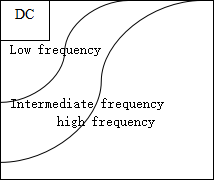
\includegraphics[width=0.3\textwidth]{Figure/2.png}
    \caption{Discrete Cosine Transform band distribution}
    \label{fig:2-2}
\end{figure}

\section{Walsh Transform}

The transformation matrix of the Walsh Transform is simple, only 1 and -1, which takes up less storage space, is easy to generate, has a fast algorithm, is widely used in image processing problems for processing large amounts of data in real time[9]. The Walsh Transform only needs to perform real-number operations, the stroage capacity is much less than the Fast Fourier Transfrom, so the operation speed is much faster. It is better than Fast Fourier Transform to use it to approximate the digital pulse signal data. The Walsh Transform has the characteristics of energy concentration, the more uniform the data distribution in the original data, the more data is concentrated on the corners of the matrix. Therefore, Walsh Transform is widely used in the fields of image transmission, telecommunication technology, and data compression.and so on.

%添加表格的方法
\begin{table}[htbp]
    \centering
    \caption{Your table caption}
    \label{tab:2-1}
    \begin{tabular}{ccc} %三列表格，全部居中
        \toprule % 顶部横线
        Header 1 & Header 2 & Header 3 \\
        \midrule % 中部横线
        Data 1 & Data 2 & Data 3 \\
        Data 4 & Data 5 & Data 6 \\
        \bottomrule % 底部横线
    \end{tabular}
\end{table}

%添加空白页，根据需要灵活取舍
\clearpage
\null
\clearpage
	\chapter{\protect\hyperlink{:}{Conclusion}}
\addtocontents{toc}{\protect\hypertarget{:}{}} %用\hypertarget实现反向跳转
\thispagestyle{fancy} % 强制当前页（第一页）使用 fancy 样式
Digital images are ubiquitous in people's lives, and images bring convenience to people's daily life, entertainment, and work. Image processing is also inseparable from people's lives. The application of image processing technology can be seen in various fields. The wider application field makes the requirements of digital image processing technology higher. People hope that more convenient, fast and real-time to acquisit and process more images, this means requiring constant research on digital image processing technology. With the continuous advancement in the field of computer technology and mathematics, the system of digital image processing systems will continue to improve.

This paper mainly introduces the four orthogonal transforms used in image processing, which is an important basic knowledge of image processing. Taking image processing as the background, from the perspective of principle, four basic transformation methods, which are Fourier Transform, Discrete Cosine Transform, Walsh Transform and Wavelet Transform, are introduced in the field of digital image processing, introduced their principles and performance separately. The four orthogonal transform algorithms are studied, and their processing in the frequency domain is realized in Matlab simulation software. The actual effects are compared by selecting image denoising and image compression in practical applications.

Through the theoretical study, actual simulation operation and comparison of results in the thesis, I have a certain understanding of the advantages of orthogonal transform in the transform domain and their practical application in image processing. The practise of algorithm simulation of orthogonal transform also helped me conceptually consolidate the relevant knowledge of orthogonal transformation. Fourier Transform has fast algorithm, which is most commonly used in digital image processing and requires complex operations. After the conversion, only the frequency domain components are included. After the centralization, the low frequency components are in the middle of the spectrogram, and the high frequency components are around the spectrogram. Discrete Cosine Transforms have fast algorithms that only require real operations. The conversion domain only contains the frequency domain components, and the low frequency components are concentrated in the upper left of the spectrum map, and the higher the frequency to the lower right. Achieve good information compression. Walsh Hadamard Transform is useful in hardware implementation of digital image processing. Easy to simulate but difficult to analyze. It is used in image data compression, filtering, and encoding. Wavelet Transform is a novel transformation method in digital image processing. After the conversion domain, there are not only the frequency domain components but also the spatial domain components, so it is called the wavelet domain. The wavelet domain contains different resolutions to obtain subbands, and the resolution to the upper left corner is smaller. There is a big advantage in image compression, and image loss is small.

I believe that in the future, with the advancement of computer technology and the emergence of more theories and algorithms, image processing technology will move toward faster, higher quality and higher intelligence.
%添加空白页，根据需要灵活取舍
\clearpage
\null
\clearpage
	\newpage

\phantomsection  % 自动生成无名锚点
%
\renewcommand{\bibname}{\protect\hyperlink{:}{Reference}}
\addtocontents{toc}{\protect\hypertarget{:}{}} %用\hypertarget实现反向跳转
\addcontentsline{toc}{chapter}{Reference}
\thispagestyle{fancy} % 强制当前页（第一页）使用 fancy 样式
\bibliographystyle{ieeetr}
\normalem	% 去掉下划线
\nocite{*}	% 引用未被引用的文献
%
\bibliography{refence/refences}  % 引用参考文献的文件

%添加空白页，根据需要灵活取舍
\clearpage
\null
\clearpage

%相关研究\cite{ref1}和\cite{ref2,ref3}表明XXX。
%\begin{thebibliography}{99}  %99表示参考文献的最大个数为99
%	\thispagestyle{fancy} % 强制当前页（第一页）使用 fancy 样式、
%	
%	\bibitem{ref1}Zheng L, Wang S, Tian L, et al., Query-adaptive late fusion for image search and person re-identification, Proceedings of the IEEE Conference on Computer Vision and Pattern Recognition, 2015: 1741-1750.  
%	\bibitem{ref2}Arandjelović R, Zisserman A, Three things everyone should know to improve object retrieval, Computer Vision and Pattern Recognition (CVPR), 2012 IEEE Conference on, IEEE, 2012: 2911-2918.  
%	\bibitem{ref3}Lowe D G. Distinctive image features from scale-invariant keypoints, International journal of computer vision, 2004, 60(2): 91-110.  
%\end{thebibliography}
	\newpage
\phantomsection  % 自动生成无名锚点
\chapter*{\protect\hyperlink{:}{Acknowledgement}}
\addcontentsline{toc}{chapter}{Acknowledgement}
\addtocontents{toc}{\protect\hypertarget{:}{}} %用\hypertarget实现反向跳转
\thispagestyle{fancy} % 强制当前页（第一页）使用 fancy 样式
% 为无编号章节手动设置页眉标记，避免沿用上一章标题
\markboth{Acknowledgement}{Acknowledgement}

Four years of university life represents a period of end, and it is a new beginning. I have a lot of words to say to people around me. When I finished this paper, the first time was a feeling of relief, and then there was a lot of thoughts.

The first thing I want to mention is my supervisor, Zhou Jingjing. I would like to thank the tutor for the advancement and guidance of my work in the overall study of the thesis, and a careful review during the completion of the thesis. Although the contact with the instructor is not long, the instructor's concern for the progress of our team's work, and the guidance of each member's work content in the group, let us work hard to complete the individual learning tasks. The mentor's enthusiasm and relaxation, and the relaxed learning style, allowed me to develop the ability of independent study and hands-on practice, which made me very productive. At the same time, the other teachers of the set up group also put forward their opinions and suggestions during the process of completing the inspection. Their supervision and supervision also remind me to remind myself to work hard to complete my task.

In addition, I would also like to thank the teachers and students who have met in this university for four years, especially my roommates and Zhang Xin teacher. You are giving me the care and life care, giving me care and encouragement when I am in trouble, sharing and communicating together when I am happy. In the process of completing the thesis, learn to share the use of new software and delve into the theoretical knowledge. It is you who let me study or live, full of optimistic attitude and caring gratitude.

I also want to thank my parents. You have always been full of tolerance and love for me, giving support to all aspects of my study and life, giving me free space that no one else has. I am grateful to my parents for urging and supporting me in the process of completing the thesis. Drinking water as a source of thought, I should present this paper as a final answer to the university and present it to you.

I am grateful to everyone around me, and I am grateful for the many things I have experienced. I will keep it in mind. What I learned during this graduation project will be my greatest asset. Finally, once again, I would like to express my heartfelt thanks to my family, classmates and teachers during the completion of the thesis!
%添加空白页，根据需要灵活取舍
\clearpage
\null
\clearpage
	\newpage
% \addcontentsline{toc}{section}{参考文献}


\chapter*{\protect\hyperlink{:}{Appendix}}
\addcontentsline{toc}{chapter}{Appendix}
\addtocontents{toc}{\protect\hypertarget{:}{}} %用\hypertarget实现反向跳转
\thispagestyle{fancy} % 强制当前页（第一页）使用 fancy 样式
% 设置附录 A 页眉标记
\markboth{Appendix}{Appendix}
Appendix 1：Fourier Transform Spectrum

clear all;close all;clc;
% Image Fourier Transform

C=fft2(im2double(I)); 

B=fftshift(C); % Move the DC component to the center of the spectrogram

D=ifft2(B); % Inverse Fourier Transform
% Display image

subplot(221);imshow(I);title('original image');

subplot(222);imshow(log(abs(C)+1),[]);title('Fourier transform uncentralized spectrogram');

subplot(223);imshow(log(abs(B)+1),[]);title('Fourier transform centralized spectrogram');

subplot(224);imshow(abs(D),[]);title('Inverse Fourier transform');
% abs modulo value display image
% log logarithmically drops the data between 0-255

	
\end{document}
